\documentclass[12pt]{article}

\usepackage{verbatim}
\usepackage{amsmath, amssymb, amsthm}
\usepackage{qtree}
\usepackage{enumerate}
\usepackage{changepage}
\usepackage{tikz}
\usetikzlibrary{arrows}
\usetikzlibrary{automata}
\usepackage{subfigure}
\usepackage{pgfplots}

\usepackage[utf8]{inputenc}

\title{CS325 Winter 2013: HW 3}
\author{
    Daniel Reichert \\
    Trevor Bramwell \\
    Lance Stringham
}
\date{\today}

\newcommand{\BigO}[1]{\ensuremath{O(#1)}}

% Big O: \BigO
% Big Omega: \Omega
% Big Theta: \Theta

% Examples:
%
%   $\BigO{n}$
%   $\Omega(n\log{n})$
%   $\Theta(\log{2n})$


\begin{document}
\maketitle

\section*{4.1}
\paragraph{Problem:}
Suppose Dijkstra\'s algorithm is run on the following graph, starting at node A.

\begin{center}
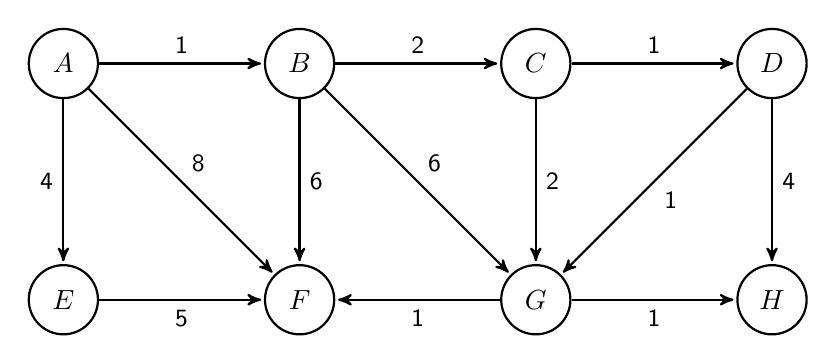
\begin{tikzpicture}[->,>=stealth',shorten >=1pt,auto,node distance=3cm,
  thick,main node/.style={font=\sffamily\bfseries}]

  \node[state] (a) {$A$};
  \node[state] (b) [right of=a]{$B$};
  \node[state] (c) [right of=b]{$C$};
  \node[state] (d) [right of=c]{$D$};
  \node[state] (e) [below of=a]{$E$};
  \node[state] (f) [below of=b]{$F$};
  \node[state] (g) [below of=c]{$G$};
  \node[state] (h) [below of=d]{$H$};
 
  \path[every node/.style={font=\sffamily\small}]
    (a) edge node [above] {1} (b)
        edge node [left] {4} (e)
        edge node {8} (f)
    (b) edge node [above] {2} (c)
        edge node [right] {6} (f)
        edge node {6} (g)
    (c) edge node [above] {1} (d)
        edge node [right] {2} (g)
    (d) edge node [right] {4} (h)
        edge node {1} (g)
    (e) edge node [below] {5} (f)
    (g) edge node [below] {1} (f)
	edge node [below] {1} (h);
\end{tikzpicture}
\end{center}

\begin{enumerate}[(a)]
    \item Draw a table showing the intermediate distance values of all
          the nodes at each iteration of the algorithm.
    \item Show the final shortest-path tree.
\end{enumerate}

\newpage
\paragraph{Solution:}
\subparagraph{(a)}

\begin{center}
\begin{tabular}{ | c | c | c | c | c | c | c | c | }
\hline
& \multicolumn{7}{|c|}{Iteration} \\ \hline
Node & 0 & 1 & 2 & 3 & 4 & 5 & 6 \\ \hline \hline
$A$ & 0 & 0 & 0 & 0 & 0 & 0 & 0 \\ \hline
$B$ & 1 & 1 & 1 & 1 & 1 & 1 & 1 \\ \hline
$C$ & $\infty$ & 3 & 3 & 3 & 3 & 3 & 3 \\ \hline
$D$ & $\infty$ & $\infty$ & 4 & 4 & 4 & 4 & 4\\ \hline
$E$ & 4 & 4 & 4 & 4 & 4 & 4 & 4 \\ \hline
$F$ & 8 & 7 & 7 & 7 & 7 & 6 & 6 \\ \hline
$G$ & $\infty$ & 7 & 5 & 5 & 5 & 5 & 5 \\ \hline
$H$ & $\infty$ & $\infty$ & $\infty$ & 8 & 8 & 6 & 6 \\
\hline
\begin{tabular}{ | c | c | c | c | c | c | c | c | c | c | }
\hline
Iteration & Node a  & Node b & Node c & Node d & Node e & Node f & Node g & Node h & Set S\\ \hline
0 & 0 & $\infty$ & $\infty$ & $\infty$ & $\infty$ & $\infty$ & $\infty$ & $\infty$ & a\\
1 & 0 & 1 & $\infty$ & $\infty$ & 4 & 8 & $\infty$ & $\infty$ & a,b\\
2 & 0 & 1 & 3 & $\infty$ & 4 & 7 & 7 & $\infty$ & a,b,c\\
3 & 0 & 1 & 3 & 4 & 4 & 7 & 5 & $\infty$ & a,b,c,d\\
4 & 0 & 1 & 3 & 4 & 4 & 7 & 5 & 8 & a,b,c,d,e\\
5 & 0 & 1 & 3 & 4 & 4 & 6 & 5 & 6 & a,b,c,d,e,g\\
6 & 0 & 1 & 3 & 4 & 4 & 6 & 5 & 6 & a,b,c,d,e,f,g\\
7 & 0 & 1 & 3 & 4 & 4 & 6 & 5 & 6 & a,b,c,d,e,f,g,h\\
\hline

\end{tabular}
\end{center}

\subparagraph{(b)}

\begin{center}
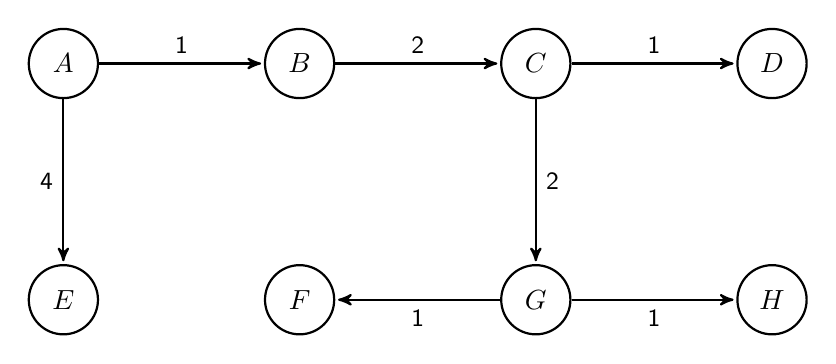
\begin{tikzpicture}[->,>=stealth',shorten >=1pt,auto,node distance=3cm,
  thick]

  \node[state] (a) {$A$};
  \node[state] (b) [right of=a]{$B$};
  \node[state] (c) [right of=b]{$C$};
  \node[state] (d) [right of=c]{$D$};
  \node[state] (e) [below of=a]{$E$};
  \node[state] (f) [below of=b]{$F$};
  \node[state] (g) [below of=c]{$G$};
  \node[state] (h) [below of=d]{$H$};
 
  \path[every node/.style={font=\sffamily\small}]
    (a) edge node [above] {1} (b)
        edge node [left]  {4} (e)
    (b) edge node [above] {2} (c)
    (c) edge node [above] {1} (d)
        edge node [right] {2} (g)
    (g) edge node [below] {1} (h)
        edge node [below] {1} (f);   
\end{tikzpicture}
\end{center}

\section*{5.2}
\paragraph{Problem:}
Suppose we want to find the minimum spanning tree of the following graph.

\begin{center}
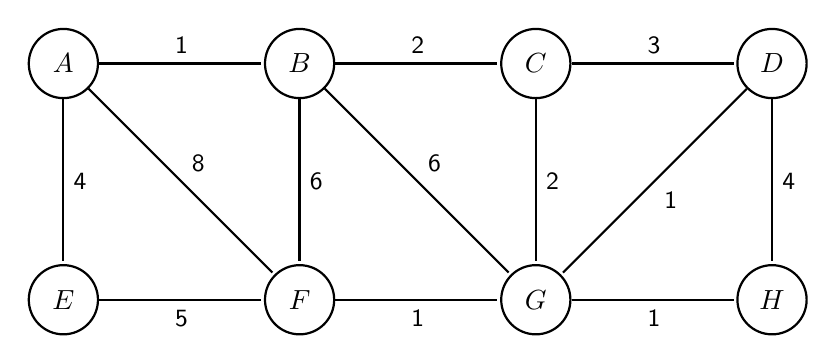
\begin{tikzpicture}[-,shorten >=1pt,auto,node distance=3cm,thick]
  \node[state] (a) {$A$};
  \node[state] (b) [right of=a]{$B$};
  \node[state] (c) [right of=b]{$C$};
  \node[state] (d) [right of=c]{$D$};
  \node[state] (e) [below of=a]{$E$};
  \node[state] (f) [below of=b]{$F$};
  \node[state] (g) [below of=c]{$G$};
  \node[state] (h) [below of=d]{$H$};

  \path[every node/.style={font=\sffamily\small}]
    (a) edge node {1} (b)
        edge node {8} (f)
        edge node {4} (e)
    (b) edge node {2} (c)
        edge node {6} (g)
        edge node {6} (f)
    (c) edge node {3} (d)
        edge node {2} (g)
    (d) edge node {1} (g)
        edge node {4} (h)
    (e) edge node [below] {5} (f)
    (f) edge node [below] {1} (g)
    (g) edge node [below] {1} (h);
\end{tikzpicture}
\end{center}

\begin{enumerate}[(a)]
\item Run Prim’s algorithm; whenever there is a choice of nodes, always
      use alphabetic ordering (e.g., start from node $A$). Draw a table showing
      the intermediate values of the cost array.

\item Run Kruskal’s algorithm on the same graph. Show how the
      disjoint-sets data structure looks at every intermediate stage
      (including the structure of the directed trees), assuming path
      compression is used.
\end{enumerate}

\paragraph{Solution:}
\subparagraph{(a)}

\begin{center}
\begin{tabular}{ | c | c | c | c | c | c | c | c | c |}
\hline
Set $S$ & $A$ & $B$ & $C$ & $D$ & $E$ & $F$ & $G$ & $H$ \\ \hline
\{\} & 0/nil & $\infty$/nil & $\infty$/nil & $\infty$/nil & $\infty$/nil
& $\infty$/nil & $\infty$/nil & $\infty$/nil \\ \hline
$A$ & & 1/$A$ & $\infty$/nil & $\infty$/nil & 4/$A$ & 6/$B$ & 6/$B$ & $\infty$/nil \\ \hline
$A,B$ & & & 2/$B$ & $\infty$/nil & 4/$A$ & 6/$B$ & 2/$C$ & $\infty$/nil \\ \hline
$A,B,C$ & & & & 3/$C$ & 4/$A$ & 6/$B$ & 2/$C$ & $\infty$/nil \\ \hline
$A,B,C,D$ & & & & & 4/$A$ & 6/$B$ & 1/$D$ & 4/$D$ \\ \hline
$A,B,C,D,E$ & & & & & & 5/$E$ & 1/$D$ & 4/$D$ \\ \hline
$A,B,C,D,E,F$ & & & & & & & 1/$D$ & 4/$D$ \\ \hline
$A,B,C,D,E,F,G$ & & & & & & 1/$G$ & & 1/$G$ \\ \hline
$A,B,C,D,E,F,G,H$ & & & & & & & & 1/$G$ \\ \hline
\end{tabular}
\end{center} 

\subparagraph{(b)}

\setlength{\belowcaptionskip}{1em}
\begin{center}
\begin{figure}
\centering
\caption{After makeset($A$), makeset($B$),\dots,makeset($H$):}
    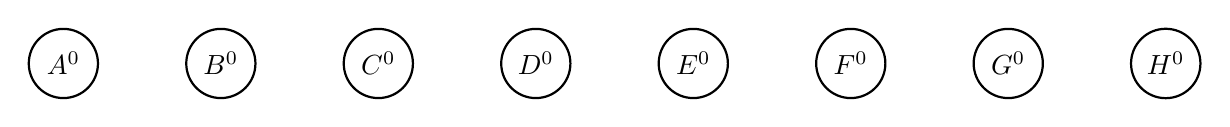
\begin{tikzpicture}[->,shorten >=1pt,auto,node distance=2cm,thick]
      \node[state] (a) {$A^0$};
      \node[state] (b) [right of=a]{$B^0$};
      \node[state] (c) [right of=b]{$C^0$};
      \node[state] (d) [right of=c]{$D^0$};
      \node[state] (e) [right of=d]{$E^0$};
      \node[state] (f) [right of=e]{$F^0$};
      \node[state] (g) [right of=f]{$G^0$};
      \node[state] (h) [right of=g]{$H^0$};
    \end{tikzpicture}
\end{figure}

\begin{figure}
\centering
\caption{After union($A$,$B$), union($G$,$F$), union($G$,$D$), union($G$,$H$):}
    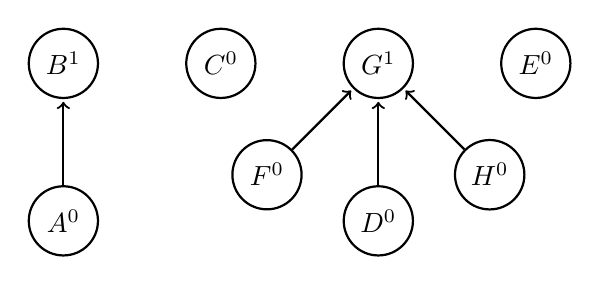
\begin{tikzpicture}[->, shorten >=1pt, auto, node distance=2cm, thick]
        \node[state] (a) {$A^0$};
        \node[state] (b) [above of=a]{$B^1$};
        \node[state] (c) [right of=b]{$C^0$};
        \node[state] (g) [right of=c]{$G^1$};
        \node[state] (f) [below left of=g]{$F^0$};
        \node[state] (d) [below of=g]{$D^0$};
        \node[state] (h) [below right of=g]{$H^0$};
        \node[state] (e) [right of=g]{$E^0$};

        \path (a) edge (b)
              (f) edge (g)
              (d) edge (g)
              (h) edge (g);
    \end{tikzpicture}
\end{figure}

\begin{figure}
\centering
\caption{After union($C$,$B$):}

    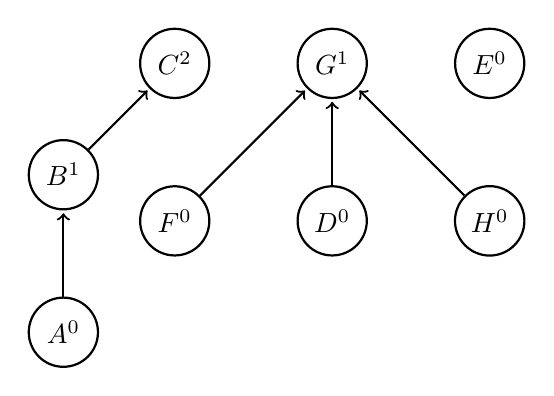
\begin{tikzpicture}[->, shorten >=1pt, auto, node distance=2cm, thick]
        \node[state] (c) {$C^2$};
        \node[state] (b) [below left of=c]{$B^1$};
        \node[state] (a) [below of=b]{$A^0$};
        \node[state] (g) [right of=c]{$G^1$};
        \node[state] (f) [below of=c]{$F^0$};
        \node[state] (d) [below of=g]{$D^0$};
        \node[state] (h) [right of=d]{$H^0$};
        \node[state] (e) [right of=g]{$E^0$};

        \path (a) edge (b)
              (b) edge (c)
              (f) edge (g)
              (d) edge (g)
              (h) edge (g);
    \end{tikzpicture}
\end{figure}

\begin{figure}
\centering
\caption{After union($G$,$C$):}
    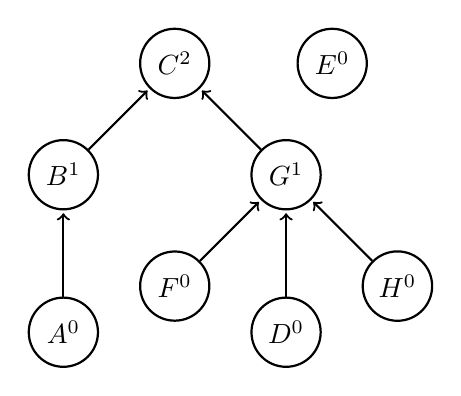
\begin{tikzpicture}[->, shorten >=1pt, auto, node distance=2cm, thick]
        \node[state] (c) {$C^2$};
        \node[state] (b) [below left of=c]{$B^1$};
        \node[state] (a) [below of=b]{$A^0$};
        \node[state] (g) [below right of=c]{$G^1$};
        \node[state] (f) [below left of=g]{$F^0$};
        \node[state] (d) [below of=g]{$D^0$};
        \node[state] (h) [below right of=g]{$H^0$};
        \node[state] (e) [right of=c]{$E^0$};

        \path (a) edge (b)
              (b) edge (c)
              (f) edge (g)
              (d) edge (g)
              (h) edge (g)
              (g) edge (c);
    \end{tikzpicture}
\end{figure}

\begin{figure}
\centering
\caption{After union($E$,$A$):}
    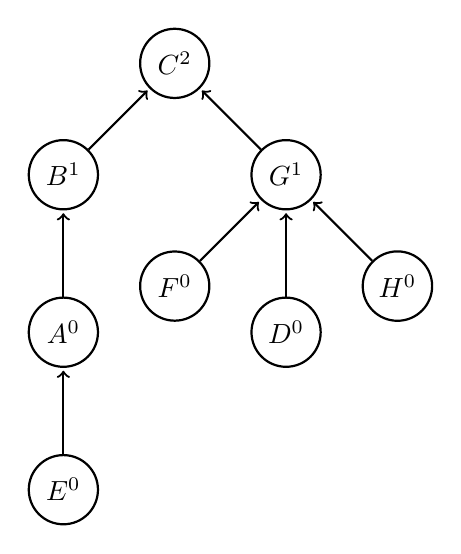
\begin{tikzpicture}[->, shorten >=1pt, auto, node distance=2cm, thick]
        \node[state] (c) {$C^2$};
        \node[state] (b) [below left of=c]{$B^1$};
        \node[state] (a) [below of=b]{$A^0$};
        \node[state] (g) [below right of=c]{$G^1$};
        \node[state] (f) [below left of=g]{$F^0$};
        \node[state] (d) [below of=g]{$D^0$};
        \node[state] (h) [below right of=g]{$H^0$};
        \node[state] (e) [below of=a]{$E^0$};

        \path (a) edge (b)
              (e) edge (a)
              (b) edge (c)
              (f) edge (g)
              (d) edge (g)
              (h) edge (g)
              (g) edge (c);
    \end{tikzpicture}
\end{figure}
\end{center}

\section*{5.5}
\paragraph{Problem:}

Consider an undirected graph $G = (V, E)$ with nonnegative edge weights
$ w_e \ge 0$. Suppose that you have computed a minimum spanning tree of
G, and that you have also computed shortest paths to all nodes from a
particular node $s \in V$.  Now suppose each edge weight is increased by
1: the new weights are $w_e = w_e + 1$.

\begin{enumerate}[(a)]
\item Does the minimum spanning tree change? Give an example where it
      changes or prove it cannot change.
\item Do the shortest paths change? Give an example where they change or
      prove they cannot change.
\end{enumerate}

\paragraph{Solution:}
\begin{proof}
Part B:  Proof by counter example.
Consider the graph:

\begin{center}
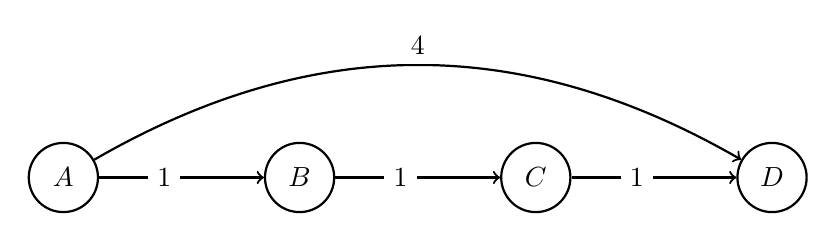
\begin{tikzpicture}[->,auto,node distance=3cm,thick]
  \tikzset{every node/.style={fill=white}} 

  \node[state] (a) {$A$};
  \node[state] (b) [right of=a]{$B$};
  \node[state] (c) [right of=b]{$C$};
  \node[state] (d) [right of=c]{$D$};
 
  \path (a) edge node [left] {$1$} (b)
        (b) edge node [left] {$1$} (c)
        (c) edge node [left] {$1$} (d);

  \path[in=150,out=30] (a) edge node {$4$} (d);
\end{tikzpicture}
\end{center}

In this graph the shortest path from A to D is from A to B to C to D
with a weight of 3. Now consider the same graph, but with all of the
edges having a weight increased by 1.

\begin{center}
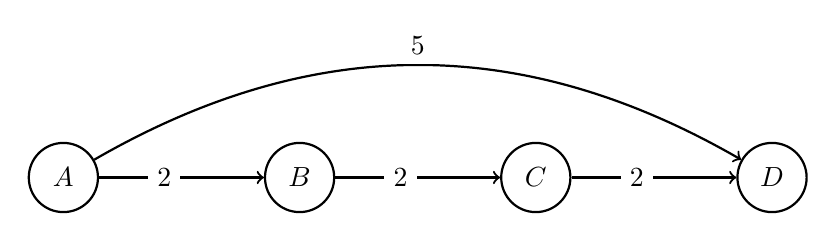
\begin{tikzpicture}[->,auto,node distance=3cm,thick]
  \tikzset{every node/.style={fill=white}} 

  \node[state] (a) {$A$};
  \node[state] (b) [right of=a]{$B$};
  \node[state] (c) [right of=b]{$C$};
  \node[state] (d) [right of=c]{$D$};
 
  \path (a) edge node [left] {$2$} (b)
        (b) edge node [left] {$2$} (c)
        (c) edge node [left] {$2$} (d);

  \path[in=150,out=30] (a) edge node {$5$} (d);
\end{tikzpicture}
\end{center}

The previously shortest path now has a weight of 6, where the direct
route from A to D only has a weight of 5.  Thus the shortest path has
changed and the counter example is proved.
\end{proof}

\begin{proof}
Part A:
Creating a shortest path tree can be thought of as distances from one node to another.  The distance formula can be derived with the use of triangles.  In uniformly increasing the weight of the edges of triangles, the ratio of the edges change. Hence it is possible, as we have just demonstrated, to have the shortest path tree change when uniformly increasing the weight of all edges.  The minimal spanning tree however, can be thought of as the balance in a graph.  Since increasing the graph uniformly does not alter the balance, we know that the minimal spanning tree will not change.

\end{proof}


\section*{5.7}
\paragraph{Problem:}
Show how to find the \emph{maximum} spanning tree of a graph, that is, the spanning tree of largest
total weight.

\paragraph{Solution:}
\begin{proof}
This can be accomplished in a similar way that a minimal spanning tree of a graph is created.  Of course there must be a difference to achieve this, and we can choose one of two options.  We can select the maximal instead of minimal edge at every iteration, or we can make all of the edge weights negative and use an existing algorithm.
\end{proof}

\section*{5}
\paragraph{Problem:}
Consider the Change Problem in Austria. The input to this problem is
an integer $L$. The output should be the minimum cardinality collection
of coins required to make $L$ shillings of change (that is, you want to use
as few coins as possible). In Austria the coins are worth 1, 5, 10, 20, 25,
50 Shillings. Assume that you have an unlimited number of coins of each
type. Formally prove or disprove that the greedy algorithm (that takes as
many coins as possible from the highest denominations) correctly solves
the Change Problem. So for example, to make change for 234 Shillings the
greedy algorithms would take four 50 shilling coins, one 25 shilling coin,
one 5 shilling coin, and four 1 shilling coins.

\paragraph{Solution:}
\begin{proof}
Proof by counter example.
When the Shilling total is equal to 40, the optimal solution would use two 20 shilling coins, so $n=2$ where $n$ is the number of coins.  According to the greedy method of taking as many coins as possible from the highest denomination available, a shilling total of 40 would have change made with one 25 shilling coin, one 15 shilling coin, and one 5 shillingcoin making $n=3$ which is not optimal.
\end{proof}

\section*{6}
\paragraph{Problem:}
Consider a long quiet country road with houses scatter very sparsely along
it (We can picture the road as a long line segment). You want to place cell
phone base stations at certain points along the road, so that every house
is within four miles of one of the base stations.
Give an efficient algorithm that achieves this goal, using as few stations
as possible. Show that the algorithm achieve the optimal solution using
the “stay ahead” argument.

\paragraph{Solution:}
\begin{proof}
Approaching from the Left or from the Right,
While:
        At the first house that you come accross that is uncovered, add four miles and place a tower

Let $T_g(i)$ denote the total number of houses covered by the first i base stations when approached from left to right in the greedy algorithm.
Let $T_o(i)$ denote the total number of houses covered by the first i base stations when approached from left to right in the optimal algorithm.
"Greedy statys ahead"
Theorem: $T_g(i) \gte T_o(i)$
If the theorem is true, then $T_g$ is optimal.

Base case: i = 1
$T_g(1) \gte T_o(1)$ is true because the greedy algorithm is creating maximal coverage with the first tower that is placed at mile j.  Any other tower placement would have less coverage, and therefore would be open to a counter example.

Because the only other placements of the base stations would either be to the west of j (there may be a house in between j and j+4 that didnt get covered), or east of j (the first house is not covered => optimatl is infesible)

Inductive step:
        Assume: $T_g(k) \gte T_o(k) \forall k \lte i$
        Prove: $T_g(k+1) \gte T_o(k+1)$

We know $T_g(k) \gte T_o(k)$.
The k base station of $T_g$ is placed at x, and $T_o$ is placed at y.
We know that $x \gte y$ from the greedy statys ahead theorem.
//this boils down to the same argument as the camping trip problem
This means that the starting point of x is at least as far as y, and will either continually tie y or exceed y.
By the inductive assumption we have that $x \gte y$.  Now let $x*$ be the k+1th base station of greedy.  Let $y*$ be the k+1th base station of $T_o$.  Because $x \gte y$ the only possibility is for x* to be at least as far as y*.  This means that $T_g(k+1) \gte T_o(k+1)$.  By induction, $T_g$ is optimal.

\end{proof}
\end{document}
